\documentclass[tikz,border=5pt]{standalone}
\usepackage{fontspec}
\setmainfont{Times New Roman}
\usepackage{unicode-math}
\setmathfont{Cambria Math}
\usetikzlibrary{shapes.geometric,positioning,fit,backgrounds,arrows.meta,calc}

\begin{document}
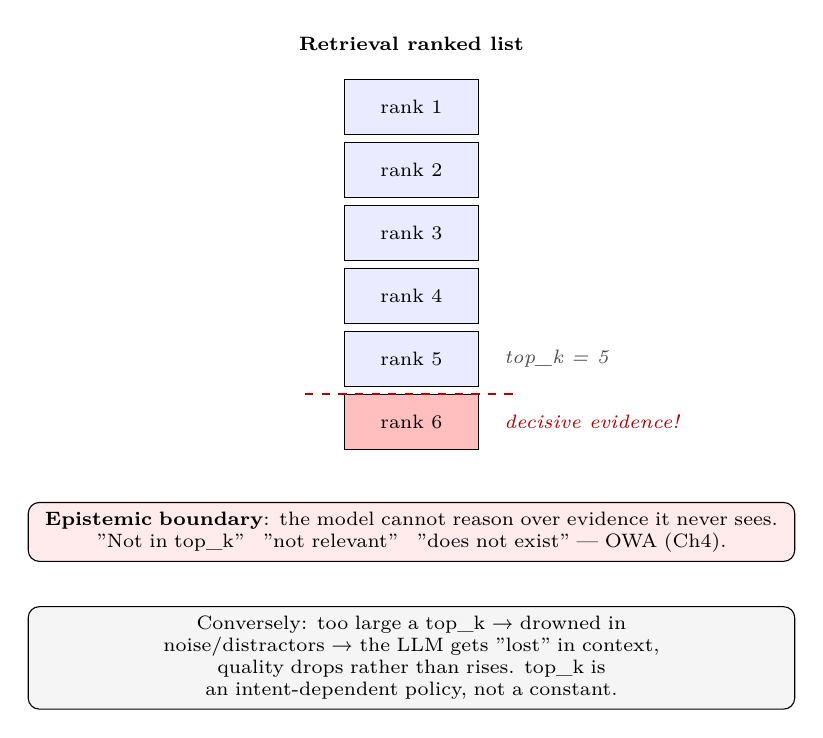
\begin{tikzpicture}[
  cell/.style={rectangle, draw, minimum width=1.7cm, minimum height=0.7cm, font=\scriptsize, align=center},
  arrow/.style={-{Stealth[length=2.2mm]}, thick},
  label/.style={font=\scriptsize\itshape, text=gray!60!black},
]

% === Ranked list with top_k boundary ===
\node[font=\scriptsize\bfseries] at (0, 2.9) {Retrieval ranked list};

\node[cell, fill=blue!8] (r1) at (0, 2.1) {rank 1};
\node[cell, fill=blue!8] (r2) at (0, 1.3) {rank 2};
\node[cell, fill=blue!8] (r3) at (0, 0.5) {rank 3};
\node[cell, fill=blue!8] (r4) at (0, -0.3) {rank 4};
\node[cell, fill=blue!8] (r5) at (0, -1.1) {rank 5};
\node[cell, fill=red!25] (r6) at (0, -1.9) {rank 6};

\draw[dashed, thick, red!70!black] (-1.35, -1.55) -- (1.35, -1.55);
\node[label, right=0.2cm of r5.east] (rk) {top\_k = 5};

\node[label, right=0.2cm of r6.east, text=red!70!black] (dec) {decisive evidence!};

% === Consequence box ===
\node[draw, rounded corners, fill=red!8, align=center, font=\scriptsize, text width=9.5cm] (cons) at (0, -3.3)
  {\textbf{Epistemic boundary}: the model cannot reason over evidence it never sees.\\
  "Not in top\_k" ≠ "not relevant" ≠ "does not exist" --- OWA (Ch4).};

% === Larger k caution ===
\node[draw, rounded corners, fill=gray!8, align=center, font=\scriptsize, text width=9.5cm] (more) at (0, -4.9)
  {Conversely: too large a top\_k → drowned in noise/distractors → the LLM gets "lost" in context,\\
  quality drops rather than rises. top\_k is an intent-dependent policy, not a constant.};

\end{tikzpicture}
\end{document}
